\documentclass[journal]{IEEEtran}
\ifCLASSINFOpdf
\else
\fi
\hyphenation{op-tical net-works semi-conduc-tor}


\usepackage[hidelinks]{hyperref}
\usepackage[cmex10]{amsmath}
\usepackage{amssymb,amsfonts}
\interdisplaylinepenalty=2500
\usepackage{dblfloatfix}
\usepackage{graphicx}
\usepackage{booktabs}
\usepackage{siunitx}
\usepackage[numbers,compress]{natbib}
\usepackage{texnames}
\usepackage{bm,bbm}
\usepackage{orcidlink}
\usepackage{latexsym}
\usepackage{array}
\usepackage{mathtools}
\usepackage{caption}
\usepackage{subcaption}
\usepackage{multirow}
\usepackage{multicol}
\usepackage{setspace}
\usepackage{algorithm}
\usepackage{algpseudocode}

% vec
\newcommand{\vecx}{\bm{x}}
\newcommand{\vecy}{\bm{y}}

% utils
\newcommand{\argmax}[1]{\underset{#1}{\mathrm{argmax}}}
\newcommand{\argmin}[1]{\underset{#1}{\mathrm{argmin}}}
\newcommand{\minimize}[1]{\underset{#1}{\mathrm{min}}}
\newcommand{\maximize}[1]{\underset{#1}{\mathrm{min}}}
\newcommand{\Norm}[2]{\lVert #1 \rVert}
\newcommand{\LOneNorm}[1]{\lVert #1 \rVert _1}
\newcommand{\LTwoNorm}[1]{\lVert #1 \rVert _2}
\newcommand{\LOneTwoNorm}[1]{\lVert #1 \rVert _{1,2}}
\newcommand{\TV}[1]{\mathrm{TV}(#1)}
\newcommand{\realNumber}{\mathbb{R}}
\newcommand{\intN}{\mathrm{N}}
\newcommand{\intM}{\mathrm{M}}
\newcommand{\BoxBall}{B_{\mathrm{box}}}
\newcommand{\LOneTwoBall}{B_{\ell_{1,2}}}

\newcommand{\LOneTwoNormDefinition}{\LOneTwoNorm{\vecx} \coloneq  \sum_{\mathfrak{g} \in \mathfrak{G}} \LTwoNorm{\vecx_\mathfrak{g}}}
\newcommand{\TotalVariationDefinition}{\TV{\vecx} \coloneq \LOneTwoNorm{\diffOperator \vecx} = \sum_{i=1}^{\intN} \sqrt{d_{h,i}^2 + d_{v,i}^2}}
\newcommand{\conjugateFunctionDefinition}{f^*(\vecx) \coloneq \sup_{\vecy \in \realNumber^N} \vecy^T \vecx - f(\vecy) }

% indicator function
\newcommand{\indicatorFunction}[2]{\iota_{#1}(#2)}
\newcommand{\indicatorFunctionDefinition}{\indicatorFunction{C}{\vecx} \coloneq \begin{cases} 0 & \text{if } \vecx \in C, \\ \infty & \text{otherwise}. \end{cases} }

% set
\newcommand{\LOneTwoBallSetDefinition}{\left\{ \LOneTwoNorm{\cdot} \le \alpha \right\}}

% proximity operator
\newcommand{\proximityOperator}[2]{\mathrm{prox}_{#1}\left(#2\right)}
\newcommand{\proximityOperatorDefinition}{\proximityOperator{ \gamma f }{\vecx} := \argmin{\vecy \in \realNumber^N} \ f(\vecy) + \frac{1}{2 \gamma} \LTwoNorm{\vecy - \vecx}^2 }
\newcommand{\proximityOperatorDefinitionWithConvexConjugateFunction}{\proximityOperator{ \gamma f^* }{\vecx} = \vecx - \gamma \proximityOperator{ \frac 1 \gamma f }{\frac 1 \gamma \vecx} }
\newcommand{\projBox}[1]{ P_{\BoxBall} \left( #1 \right) }
\newcommand{\projBoxSolution}{ \projBox{\vecx} = \text{min}( \text{max} (\vecx, l), u) }
\newcommand{\projLOneTwoBall}[1]{P_{\LOneTwoBall}\left(#1\right)}
\newcommand{\projLOneTwoBallSolution}{
    (\projLOneTwoBall{\vecx})_{\mathfrak{g}_i} =
        \begin{cases}
            0 & \text{if} \ \LTwoNorm{\vecx_{\mathfrak{g}_i}} = 0, \\
            \bm \beta_i \frac {\vecx_{\mathfrak{g}_i}} {\LTwoNorm{\vecx_{\mathfrak{g}_i}}} & \text{otherwise},
        \end{cases} \\
}
\newcommand{\projLOneTwoBallSolutionWhere}{
    \bm \beta = P_{ \{ \LOneNorm{ \cdot } \le \alpha \} }\left( \left[ \LTwoNorm{ \vecx_{\mathfrak{g}_1} }, \ldots, \LTwoNorm{ \vecx_{\mathfrak{g}_N} } \right]^T \right) \\
}
\newcommand{\projLOneBall}[1]{P_{ \{ \LOneNorm{ \cdot } \le \alpha \} }(#1)}
\newcommand{\projLOneBallSolution}{\projLOneBall{\vecx} = \text{SoftThrethold}(\vecx, \beta)}
\newcommand{\projLOneBallSolutionWhere}{
    \begin{aligned}
        & \bm x_{\text{abs}} = \text{abs}(\vecx), \\
        & \bm y              = \text{sort}_{\text{desc}}(\vecx_{\text{abs}}), \\
        & \beta'             = \text{max} \left\{ \frac 1 i \left(\left(\sum_{j=1}^i \bm y_j\right) - \alpha\right) \middle| \ i = 1, \ldots, N \right\}, \\
        & \beta              = \text{max} \left\{ \beta', 0 \right\}. \\
    \end{aligned}
}


% Primal-Dual Splitting
\newcommand{\PDSPrimal}{\minimize { \vecx \in \realNumber^N } \left\{ f(\vecx) + g(\vecx) + h(\bm{L} \vecx) \right\} }
\newcommand{\PDSDual}{\minimize { \vecy \in \realNumber^M } \left\{ (f+g)^*(-\bm{L}^T \vecy) + h^*(\vecy) \right\} }
\newcommand{\PDSSubStep}{
\left \lfloor \ \
    \begin{aligned}
        & \vecx^{(k+1)} = \proximityOperator{\gamma_1 g}{\vecx^{(k)} - \gamma_1( \nabla f(\vecx^{(k)}) + \bm{L}^T \vecy^{(k)} )}, \\
        & \vecy^{(k+1)} = \proximityOperator{\gamma_2 h^*}{\vecy^{(k)} + \gamma_2 \bm{L} (2\vecx^{(k+1)} - \vecx^{(k)}) }, \\
    \end{aligned}
\right.
}

% seismic + related proposed method
\newcommand{\diffOperator}{\mathbf{D}}
\newcommand{\velModel}{\bm{m}}
\newcommand{\seismicData}{\bm{u}}

% FWI objective
\newcommand{\FWIObjectiveDefinition}{ E(\velModel) = \frac {1} {2} \LTwoNorm { \seismicData_{\mathrm{obs}} - \seismicData_{\mathrm{cal}}(\velModel) }^2 }
\newcommand{\FWIGradientDefinition}{ \nabla E(\velModel) = \seismicData_{\mathrm{obs}} - \nabla \seismicData_{\mathrm{cal}(\velModel)} }
\newcommand{\FWIObjectiveWithTVConstraint}{ E(\velModel) \ \ \ \text{s.t.} \ \  \begin{cases} \LOneTwoNorm{\diffOperator \velModel} \le \alpha, \\ \velModel \in [l,u]^N, \end{cases}}
\newcommand{\FWIObjectiveWithTVConstraintWithIndicatorFunction}{ E(\velModel) + \indicatorFunction{\BoxBall}{\velModel} + \indicatorFunction{\LOneTwoBall}{\diffOperator \velModel} }

\newcommand{\FWIWithPDS}{
\left \lfloor \ \
    \begin{aligned}
        & \widetilde{\velModel} = \FWIWithPDSStepMTmp \\
        & \velModel^{(k+1)}             = \FWIWithPDSStepM \\
        & \widetilde{\vecy}     = \FWIWithPDSStepYTmp \\
        & \vecy^{(k+1)}                 = \FWIWithPDSStepY.
    \end{aligned}
\right.
}
\newcommand{\FWIWithPDSStepMTmp}{ \velModel^{(k)} - \gamma_1 \left( \nabla E(\velModel^{(k)}) + \bm{D}^T \vecy^{(k)} \right) }
\newcommand{\FWIWithPDSStepM}   { \projBox{\widetilde{\velModel}} }
\newcommand{\FWIWithPDSStepYTmp}{ \vecy^{(k)} + \gamma_2 \bm{D} \left( 2\velModel^{(k+1)} - \velModel^{(k)} \right) }
\newcommand{\FWIWithPDSStepY}   { \widetilde{\vecy} - \gamma_2 \projLOneTwoBall{\frac 1 {\gamma_2} {\widetilde{\bm y}}} }



\newcommand{\FWIWithGradient}{ \velModel^{(k+1)} = \velModel^{(k)} - \gamma \left( \nabla E(\velModel^{(k)}) \right) }





\begin{document}
    \makeatletter
\def\bstctlcite{\@ifnextchar[{\@bstctlcite}{\@bstctlcite[@auxout]}}
\def\@bstctlcite[#1]#2{\@bsphack
\@for\@citeb:=#2\do{%
\edef\@citeb{\expandafter\@firstofone\@citeb}%
\if@filesw\immediate\write\csname #1\endcsname{\string\citation{\@citeb}}\fi}%
\@esphack}
\makeatother
\bstctlcite{IEEEexample:BSTcontrol}


    \title{Efficient and Accurate Full-Waveform Inversion with Total Variation Constraint}

	\author{
        Yudai Inada, Shingo Takemoto, Student Member, IEEE, and Shunsuke Ono, Member, IEEE
%		\IEEEauthorblockN{Yudai INADA}
%		\IEEEauthorblockA{\textit{Institute of Science Tokyo}\\ inada.y.de71@m.isct.ac.jp}

%		\and

%		\IEEEauthorblockN{Shingo TAKEMOTO}
%		\IEEEauthorblockA{\textit{Institute of Science Tokyo}\\ takemoto.s.e908@m.isct.ac.jp}

%		\and

%		\IEEEauthorblockN{Shunsuke ONO}
%		\IEEEauthorblockA{\textit{Institute of Science Tokyo}\\ ono.s.5af2@m.isct.ac.jp}

		\thanks{
    Manuscript received XXX, XXX; revised XXX XXX, XXX.
}
\thanks{
    This work was supported in part by JST PRESTO under Grant JPMJPR21C4 and JST AdCORP under Grant JPMJKB2307, and in part by JSPS KAKENHI under Grant 22H03610, 22H00512, 23H01415, 23K17461, 24K03119, and 24K22291.
}
\thanks{
    Y. Inada is with the School of Computing, Institute of Science Tokyo, Yokohama, 226-8501, Japan (E-mail: inada.y.de71@m.isct.ac.jp).
}
\thanks{
    S. Takemoto is with the School of Computing, Institute of Science Tokyo, Yokohama, 226-8501, Japan (E-mail: takemoto.s.e908@m.isct.ac.jp).
}
\thanks{
    S. Ono is with the School of Computing, Institute of Science Tokyo, Yokohama, 226-8501, Japan (E-mail: ono.s.5af2@m.isct.ac.jp).
}


	}

    \markboth{IEEE Geoscience and remote sensing letters, VOL. XX, 2025}
    {Shell \MakeLowercase{\textit{et al.}}: Efficient and Accurate Full-Waveform Inversion with Total Variation Constraint}

    \maketitle

    \begin{abstract} This paper proposes a computationally efficient algorithm to address the Full-Waveform Inversion (FWI) problem with a Total Variation (TV) constraint, designed to accurately reconstruct subsurface properties from seismic data.
FWI, as an ill-posed inverse problem, requires effective regularizations or constraints to ensure accurate and stable solutions.
Among these, the TV constraint is widely known as a powerful prior for modeling the piecewise smooth structure of subsurface properties.
However, solving the optimization problem is challenging because of the nonlinear observation process combined with the non-smoothness of the TV constraint.
Conventional methods rely on inner loops and/or approximations, which lead to high computational cost and/or inappropriate solutions.
To address these limitations, we develop a novel algorithm based on a primal-dual splitting method, achieving computational efficiency by eliminating inner loops and ensuring high accuracy by avoiding approximations.
We also demonstrate the effectiveness of the proposed method through experiments using the SEG/EAGE Salt and Overthrust Models.
The source code will be available at https://www.mdi.c.titech.ac.jp/publications/fwiwtv. \end{abstract}

    \begin{IEEEkeywords} full-waveform inversion, total variation, primal-dual splitting method. \end{IEEEkeywords}

    \IEEEpeerreviewmaketitle

    \section{Introduction}      \label{sec:Introduction}    \IEEEPARstart{F}{ull-Waveform} Inversion (FWI)~\cite{FWI0,FWI1} is a technique for reconstructing subsurface properties from seismic data measured at multiple observation points.
The subsurface properties obtained through FWI are essential in geological research and resource exploration, such as locating gas and oil reservoirs, characterizing mineral deposits, and assessing groundwater flow patterns~\cite{FWI1,FWIApplicationGroundwater0,FWIApplicationGroundwater1}.
In addition to the geological field, FWI has also been successfully applied to non-destructive testing, including brain tissue analysis in medical imaging and material detection in industrial inspection ~\cite{FWIApplicationNonDestructiveTesting0,FWIApplicationNonDestructiveTesting1}.

FWI faces significant challenges in directly reconstructing subsurface properties from seismic data because of the nonlinear wave propagation and the inherent complexity of the observation process~\cite{FWI1}.
To address this issue, FWI is typically formulated as an optimization problem that minimizes the squared error between observed and simulated seismic data~\mbox{\cite{FWI0,CustomFWI0,CustomFWI1,CustomFWI2,CustomFWI3,CustomFWI4,CustomFWI5}}, which serves as the standard approach.
Nevertheless, the inherent ill-posedness of FWI necessitates the incorporation of regularization techniques.
Among these, Tikhonov regularization~\cite{tikhonov} and Total Variation (TV)-based methods~\cite{TV,TGV} are widely used to promote piecewise smoothness in the reconstructed subsurface properties, improving stability and accuracy~\cite{FWI-with-tikhonov-regularization,FWI-with-TV-regularization,FWI-with-directional-TV-regularization,FWI-with-high-order-TV-regularization,FWI-with-TGV-regularization}.
While these regularization techniques are effective, they often involve the careful tuning of a balance parameter that determines the trade-off between the FWI objective function and the regularization term.
To overcome this limitation, an alternative approach has been proposed: incorporating the TV prior as a constraint rather than as a regularization term~\cite{FWI-with-TV-constraint,FWI-with-TV-constraint2,FWI-with-TV-constraint3,FWI-with-TV-constraint4}.
This formulation decouples the parameter for the TV constraint from the FWI objective, allowing it to be determined independently based on prior knowledge of subsurface properties~\cite{constraint0,constraint1,constraint2,constraint3,constraint4,constraints-vs-penalties-in-FWI}.
By doing so, this approach not only simplifies parameter selection but also enhances the interpretability of both the mathematical formulation and the reconstructed subsurface models.

Despite its advantages, solving the TV-constrained FWI problem presents considerable difficulties due to the interplay between the nonlinear observation process and the non-smoothness of the TV term.
Conventional methods~\mbox{\cite{FWI-with-TV-constraint,FWI-with-TV-constraint2,FWI-with-TV-constraint3,FWI-with-TV-constraint4}} attempt to address these issues by incorporating inner loops to enforce the constraint at each optimization step or by employing linear or quadratic approximations.
However, these approaches come with notable drawbacks: inner loops substantially increase computational cost, and approximations compromise reconstruction accuracy.
This raises a crucial question: \textit{Is it possible to develop an algorithm that solves the TV-constrained FWI problem efficiently while avoiding inner loops and approximations?}

In this paper, we introduce a novel algorithm for solving the TV-constrained FWI problem using a primal-dual splitting method~\cite{PDS2}.
The proposed algorithm effectively addresses the intertwined issues of the nonlinear observation process and the non-smoothness of the TV constraint, achieving accurate reconstructions without relying on approximations.
Additionally, by eliminating the need for inner loops, our approach is markedly more computationally efficient than existing methods.
We validate the performance of our algorithm through numerical experiments on the SEG/EAGE Salt and Overthrust Models, demonstrating its capability to efficiently enforce the constraints while delivering high-quality reconstructions.


    \section{Preliminaries}     \label{sec:Preliminaries}   \subsection{Mathematical Tools} \label{subsec:mathematical-tools}

Throughout this paper, we denote vectors and matrices by bold lowercase letters (e.g., $\vecx$) and bold uppercase letters (e.g., $\bm{X}$), respectively.

For $\vecx \in \realNumber^{\intN}$, the mixed $\ell_{1,2}$ norm is defined as follows:
\begin{equation} \label{eq:L12NormDefinitionEq} \LOneTwoNormDefinition, \end{equation}
where $\mathfrak{G}$ is a set of disjoint index sets, and $\vecx_{\mathfrak{g}}$ is the subvector of $\vecx$ corresponding to the indices in $\mathfrak{g}$.

For $\vecx \in \realNumber^{\intN}$, the total variation (TV)~\cite{TV} is defined as follows:
\begin{equation} \label{eq:TVDefinitionEq} \TotalVariationDefinition, \end{equation}
where $d_{h,i}$ and $d_{v,i}$ are the horizontal and vertical differences of the $i$-th element of $\vecx$, respectively, when the vector $\vecx$ is considered as a matrix.



\subsection{Proximal Tools} \label{subsec:proximal-tools}

We denote the set of proper lower-semicontinuous convex functions $\realNumber^N \to (- \infty, \infty]$ by $\Gamma_0(\realNumber^N)$.

For $\gamma > 0$ and $f \in \Gamma_0(\realNumber^N)$, the proximity operator is defined as follows:
\begin{equation} \label{eq:ProximityOperatorDefinitionEq} \proximityOperatorDefinition. \end{equation}

For $f \in \Gamma_0(\realNumber^N)$, the convex conjugate function $f^*$ is defined as follows:
\begin{equation} \label{eq:ConjugateFunctionDefinitionEq} \conjugateFunctionDefinition. \end{equation}

The proximity operator of the convex conjugate function is expressed as follows~\cite[Theorem 3.1 (ii)]{prox-convex-conjugate-function}:
\begin{equation} \label{eq:ProximityOperatorDefinitionWithConvexConjugateFunctionEq} \proximityOperatorDefinitionWithConvexConjugateFunction. \end{equation}

For a nonempty closed convex set $C \subset \realNumber^N$, the indicator function $\iota_C: \realNumber^N \to (- \infty, \infty] $ is defined as follows:
\begin{equation} \label{eq:IndicatorFunctionDefinitionEq} \indicatorFunctionDefinition \end{equation}

%The proximity operator of $\iota_C$ is the projection onto $C$, given by
The proximity operator of $\iota_C$ is equivalent to the projection onto $C$, given by
\vspace{-1.4mm}
\begin{equation} \label{eq:ProximityOperatorDefinitionWithIndicatorFunctionEq}
\proximityOperator{ \gamma \iota_{C} }{\vecx} = P_C(\vecx) \coloneq \argmin{\vecy \in C} \ \LTwoNorm{\vecy - \vecx}.
\end{equation}



\subsection{Primal-Dual Splitting Algorithm} \label{subsec:primal-dual-splitting-algorithm}

The Primal-Dual Splitting algorithm (PDS)~\cite{PDS2} is applied to the following problem:
\begin{equation} \label{eq:PDSPrimalEq} \PDSPrimal, \end{equation}
where $\bm{L} \in \realNumber^{\intM \times \intN}$ is a linear operator, $f$ is a differentiable convex function and $g,h$ are convex functions whose proximity operator can be computed efficiently.

PDS solves Prob.~\eqref{eq:PDSPrimalEq} by iteratively updating the following:
\begin{equation} \label{eq:PDSSubStep} \PDSSubStep \end{equation}
where $\gamma_1, \gamma_2 > 0$ are step sizes.


\subsection{Full-Waveform Inversion (FWI)} \label{subsec:full-waveform-inversion}

Typically, FWI is treated as the following optimization problem~\cite{FWI0}:
\begin{equation} \label{eq:FWIObjective} \argmin{\velModel \in \realNumber^N} \ \ \FWIObjectiveDefinition, \end{equation}
where $\velModel \in \realNumber^{N}$ is the velocity model representing subsurface properties, $\seismicData_{\mathrm{obs}} \in \realNumber^{M}$ is the observed seismic data, $\seismicData_{\mathrm{cal}} : \realNumber^{N} \rightarrow \realNumber^{M}$ is the observation process, and $\seismicData_{\mathrm{cal}}(\velModel)$ is the modeled seismic data with the velocity model.
$N$ is the number of grid points, and $M$ is the total data size of the observed seismic data, defined as the total product of the number of waveform sources, time samples, and receivers.

The observation process $\seismicData_{\mathrm{cal}}$ is nonlinear and complex, making it difficult to analytically derive the optimal solution.
However, the gradient $\nabla E$ can be computed numerically by simulating the wave equation using the adjoint-state method~\cite{FWI-gradient}.


    \section{Proposed Method}   \label{sec:ProposedMethod}  %\input{src/img/salt-velocity-model}

We introduce the TV and box constraint into the FWI problem to achieve more accurate reconstruction.
As shown in Fig.~\ref{fig:experiment-data}, the velocity model is piecewise smooth, thus introducing the TV constraint to achieve a more accurate reconstruction.
The box constraint ensures that the velocity model remains within valid ranges.

The optimization problem of the TV and box constrained FWI is formulated as follows:
\begin{equation} \label{eq:FWIObjectiveWithTVConstraint} \argmin{\velModel \in \realNumber^N} \ \ \FWIObjectiveWithTVConstraint \end{equation}
where $\alpha \ge 0$ is the upper bound of the $\ell_{1,2}$ norm, and $u > l > 0$ are the upper and lower bounds of the velocity model values, respectively.
By incorporating TV as a constraint, the parameter $\alpha$ can be determined independently of other terms or constraints, which has been highlighted as an advantage in prior works~\cite{constraint0,constraint1,constraint2,constraint3,constraint4,constraints-vs-penalties-in-FWI}.
This separation makes it possible to directly control smoothness according to $\alpha$, providing a clearer interpretation of the reconstructed subsurface properties.

The constraints can be incorporated into the objective function as indicator functions:
\begin{equation} \label{eq:FWIObjectiveWithTVConstraintWithIndicatorFunction} \argmin{\velModel \in \realNumber^N} \ \ \FWIObjectiveWithTVConstraintWithIndicatorFunction, \end{equation}
where
\begin{equation}
    \label{eq:LOneTwoBallDefinition}
    \begin{aligned}[b]
        \BoxBall & \coloneqq [l,u]^N, \\
        \LOneTwoBall & \coloneqq \LOneTwoBallSetDefinition.
    \end{aligned}
\end{equation}


The proximity operator of $\iota_{\BoxBall}$ and $\iota_{\LOneTwoBall}$ can be computed efficiently.
Therefore, these functions of $E$, $\iota_{\BoxBall}$ and $\iota_{\LOneTwoBall}$ correspond to $f$, $g$ and $h$ in \eqref{eq:PDSPrimalEq}, respectively, $\diffOperator$ is corresponds to $\bm{L}$, so the problem~\eqref{eq:FWIObjectiveWithTVConstraintWithIndicatorFunction} can be solved using PDS.
We show the detailed algorithm in Algorithm~\ref{alg:FWIWithPDS}.
By strictly following the PDS framework, our algorithm accurately solves the optimization problem without relying on approximations or relaxations.
%\begin{equation} \label{eq:FWIWithPDS} \FWIWithPDS \notag \end{equation}
\begin{algorithm}[t]
    \caption{PDS based solver for~\eqref{eq:FWIObjectiveWithTVConstraintWithIndicatorFunction}}\label{alg:FWIWithPDS}
    \begin{algorithmic}[1]
        \Statex \textbf{Input:} $ \velModel^{(0)}, \vecy^{(0)}, \gamma_0 > 0, \gamma_1 > 0 $
        \While {A stopping criterion is not satisfied}
            \State $\widetilde{\velModel} \leftarrow \FWIWithPDSStepMTmp $
            \State $\velModel^{(k+1)}     \leftarrow \FWIWithPDSStepM $
            \State $\widetilde{\vecy}     \leftarrow \FWIWithPDSStepYTmp $
            \State $\vecy^{(k+1)}         \leftarrow \FWIWithPDSStepY $
        \EndWhile
        \Statex \textbf{Output:} $\velModel^{(k)}$
    \end{algorithmic}
\end{algorithm}


The proximity operators of $\iota_{\BoxBall}$ and $\iota_{\LOneTwoBall}$, that is, the metric projections onto $\BoxBall$ and ${\LOneTwoBall}$ are calculated by
\begin{equation} \label{eq:ProximityOperatorForBoxConstraint} \projBoxSolution, \end{equation}
\begin{equation} \label{eq:ProximityOperatorForL12Ball} \projLOneTwoBallSolution \end{equation}
where
\begin{equation} \label{eq:ProximityOperatorForL12BallWhere} \projLOneTwoBallSolutionWhere, \end{equation}
and $\mathfrak{g}_i$ is an index set corresponding to the horizontal and vertical differences of the $i$-th element of $\velModel$.
The proximity operator of the $\ell_1$-norm ball is provided in~\cite{L1-ball-projection}.
%The proximity operator for the $l_1$ norm upper bound constraint is expressed as follows~\cite{L1-ball-projection}:
%\begin{equation} \label{eq:ProximityOperatorForL1Ball}  \projLOneBallSolution, \end{equation}
%where
%\begin{equation}
%    \label{eq:ProximityOperatorForL1BallWhere}
%    \begin{aligned}[b]
%        & \bm x_{\text{abs}} = \text{abs}(\vecx), \\
%        & \bm y              = \text{sort}_{\text{desc}}(\vecx_{\text{abs}}), \\
%        & \beta'             = \text{max} \left\{ \frac 1 i \left(\left(\sum_{j=1}^i \bm y_j\right) - \alpha\right) \middle| \ i = 1, \ldots, N \right\}, \\
%        & \beta              = \text{max} \left\{ \beta', 0 \right\}. \\
%    \end{aligned}
%\end{equation}

%\subsection{Computational Cost of Our Algorithm} \label{subsec:computational-cost-of-out-algorithm}
%\vspace{2.5mm}
%\noindent \textit{Remark}: Computational Cost of Our Algorithm
%\vspace{1.5mm}

\newtheorem{theorem}{Remark}
\begin{theorem}[Computational Cost of Our Algorithm]
Our algorithm efficiently solves the optimization problem of the TV and box constrained FWI without relying on inner loops.
Thus, the iteration-dependent factor in the computational cost is eliminated, and the computational complexity to enforce the TV constraint is reduced to $O(N \log N)$, where $N$ is the number of grid points in the velocity model.
Furthermore, existing methods require a computational cost of $O(N \log N)$ or more at each inner-loop iteration, clearly demonstrating the efficiency of our approach.
Due to the reduced cost of incorporating TV constraints, the computational cost at each iteration in our algorithm is dominated by the gradient computation, $\nabla E$, which involves simulating the wave equation along the time axis.
This step has a computational complexity of $O(S\, TN)$, where $S$ is the number of waveform sources and $T$ is the number of time samples.
\end{theorem}








    \section{Experiments}       \label{sec:Experiments}     \subsection{Experimental Setup} \label{subsec:experimental-setup}

To demonstrate the effectiveness of the TV and box constrained FWI, we conducted FWI experiments where we compared with the standard FWI method\footnote{
    \begin{minipage}{0.95\linewidth}
        The standard FWI method uses the following procedures:
        \begin{equation}
            \FWIWithGradient \label{eq:FWIWithGradient}
        \end{equation}
        where $\gamma > 0$ is the step size.
    \end{minipage}
}\cite{FWI0}, using the SEG/EAGE Salt and Overthrust Models.

The velocity model consists of 50 $\times$ 100 grid points.
Fig.~\ref{fig:experiment-data} shows the ground truth velocity model and the initial velocity model, which is created by smoothing the ground truth with a Gaussian filter with a standard deviation of 80.
The source waveform is a Ricker wavelet with a peak wavelet frequency of 10 Hz.
The number of waveform sources and receivers is 20 and 101, respectively, and they are placed on the surface at equal intervals.
The gradient $\nabla E$ is computed numerically using the Devito framework~\cite{devito}.
The number of iterations is set to 5000.
Experiments are conducted with and without noise in the observed data, as shown in Fig.~\ref{fig:observed-seismic-data}.
The noise is Gaussian noise with mean 0 and variance 1.
In our algorithm, the step sizes $\gamma_1$ and $\gamma_2$ are set to $1.0 \times 10^{-4}$ and $1.0 \times 10^2$, respectively.
The lower and upper bounds of the velocity model $l$, $u$ are set to 1.5~[km/s] and 4.5~[km/s], respectively.
The experiments are conducted using $\alpha$ values ranging from 100 to 700 in steps of 50, representing the upper bound of the $\ell_{1,2}$ norm.
In the standard FWI method, the step size $\gamma$ is set to $1.0 \times 10^{-4}$.

\begin{figure}[t]
    \centering
    \begin{tabular}{m{40mm} m{40mm} m{10mm}}
        \begin{minipage}[b]{\linewidth}
            \centering
            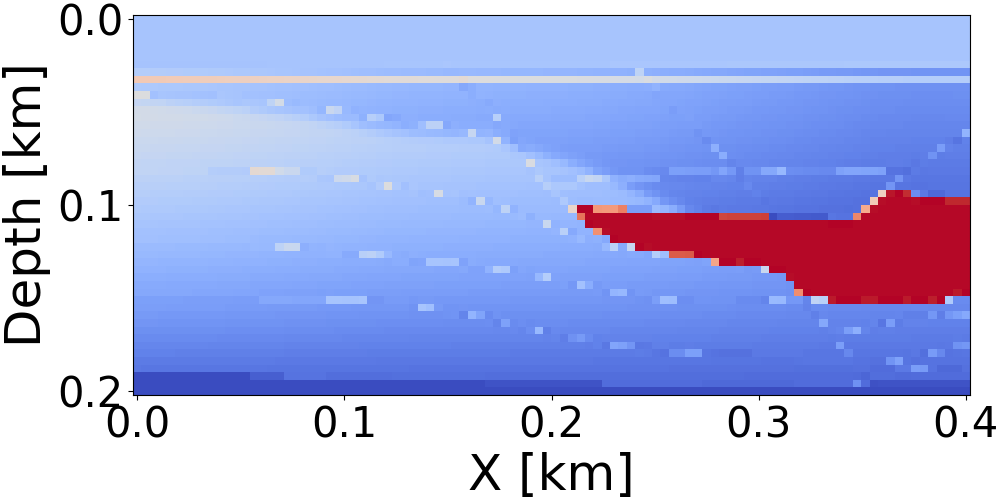
\includegraphics[width=\linewidth]{public/true}
%            \vspace{-9mm}
            \caption*{\raisebox{-3mm}{Ground truth}}
%            \vspace{1mm}
        \end{minipage} &
        \hspace{-5mm}
        \begin{minipage}[b]{\linewidth}
            \centering
            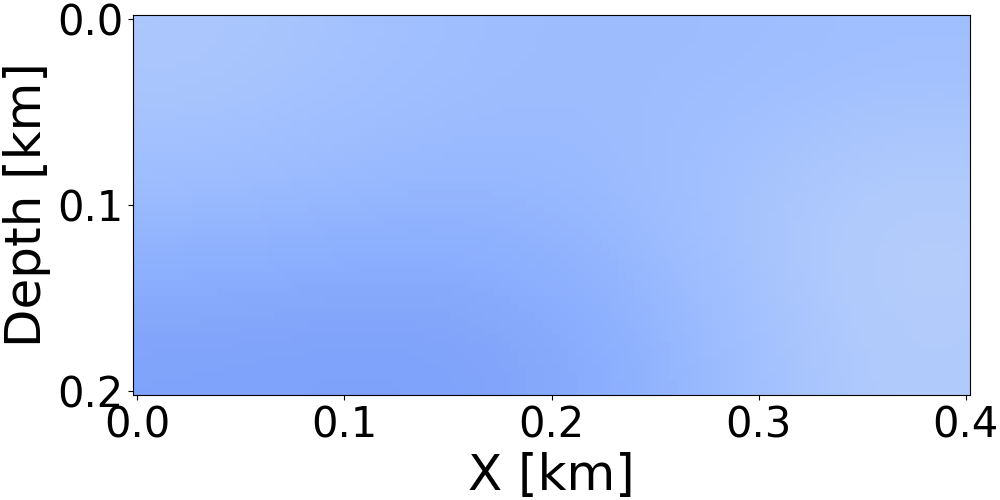
\includegraphics[width=\linewidth]{public/initial}
%            \vspace{-9mm}
            \caption*{\raisebox{-3mm}{Initial model}}
%            \vspace{1mm}
        \end{minipage} &
        \hspace{-8mm}
        \raisebox{3.5mm}{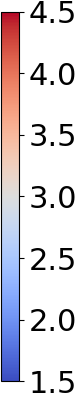
\includegraphics[height=25mm]{public/color-bar}}
    \end{tabular}
%    \vspace{-4mm}
    \caption{The velocity models for experiments.}
%    \vspace{-5mm}
    \vspace{2mm}
    \label{fig:experiment-data}
\end{figure}

\begin{figure}[t]
    \centering
    \begin{tabular}{m{3mm} m{30mm} m{30mm} m{10mm}}
        % dummy
        \begin{minipage}[b]{\linewidth}\end{minipage} &

        \begin{minipage}[b]{\linewidth}
            \centering
            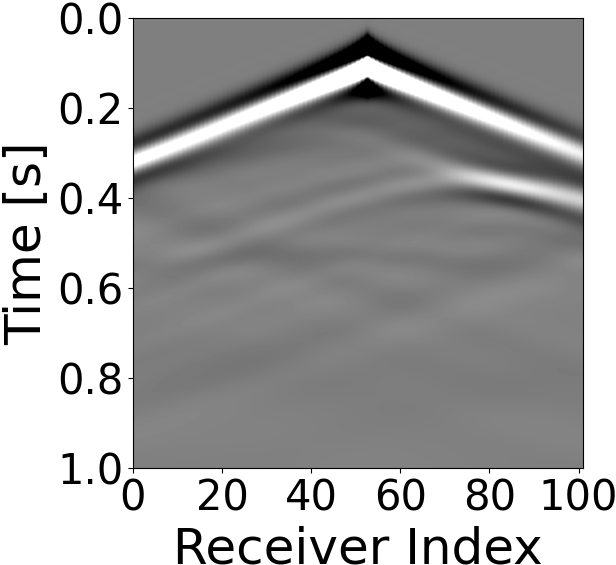
\includegraphics[width=\linewidth]{public/seismic_data}
%            \vspace{-7mm}
            \caption*{\raisebox{-2mm}{Seismic Data}}
%            \vspace{1mm}
        \end{minipage} &
        \begin{minipage}[b]{\linewidth}
            \centering
%            \vspace{1mm}
            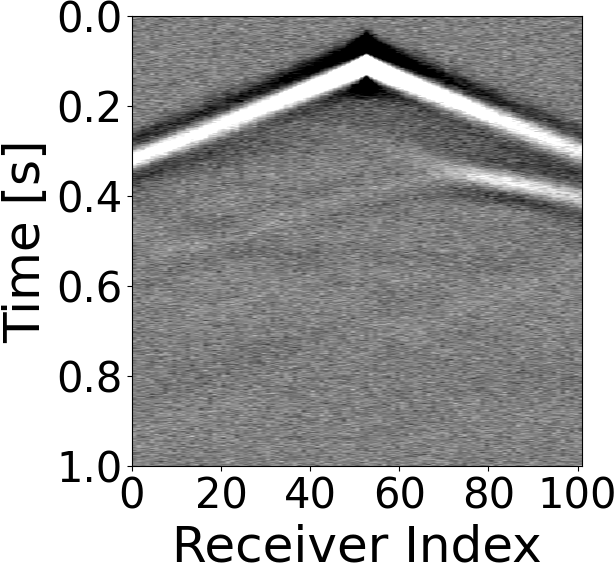
\includegraphics[width=\linewidth]{public/seismic_data_noisy}
%            \vspace{-7mm}
            \caption*{\raisebox{-2mm}{Noisy Seismic Data}}
%            \vspace{1mm}
        \end{minipage} &
        \hspace{-3mm}
        \multirow[t]{3}{*}{\raisebox{-5.8mm}{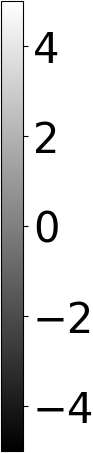
\includegraphics[height=24mm]{public/seismic-data-color-bar}}} \\
    \end{tabular}
%    \vspace{-4mm}
    \captionsetup{margin=1.3cm}
    \caption{The sinthesized seismic data \\ corresponding to a single source waveform.}
%    \vspace{-5mm}
    \label{fig:observed-seismic-data}
\end{figure}


\begin{figure*}[htbp]
    \centering
    \begin{tabular}{m{43mm} m{43mm} m{43mm} m{43mm} m{10mm}}
        \hspace{-3mm}
        \begin{minipage}[b]{\linewidth}
            \centering
            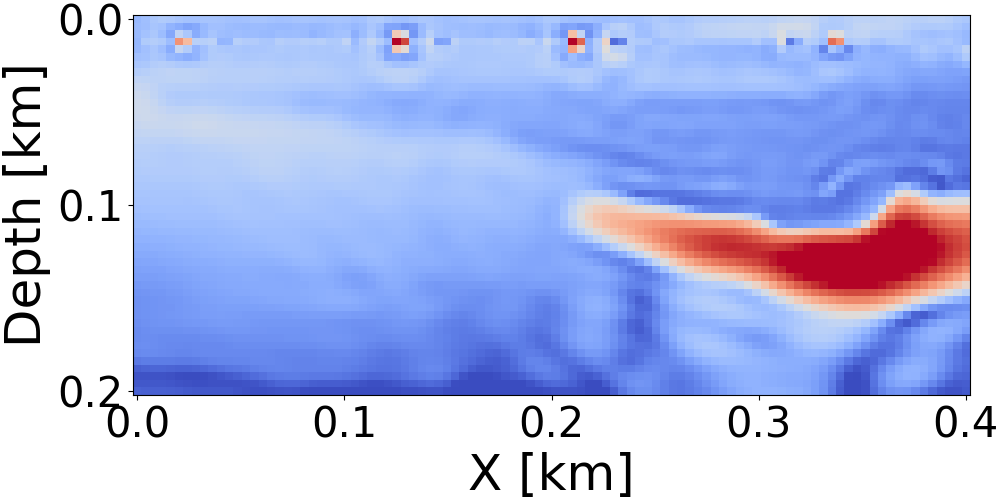
\includegraphics[width=\linewidth]{public/gradient}
%            \vspace{-6mm}
            \caption*{(a) Standard FWI}
%            \vspace{1mm}
        \end{minipage} &
        \hspace{-8mm}
        \begin{minipage}[b]{\linewidth}
            \centering
            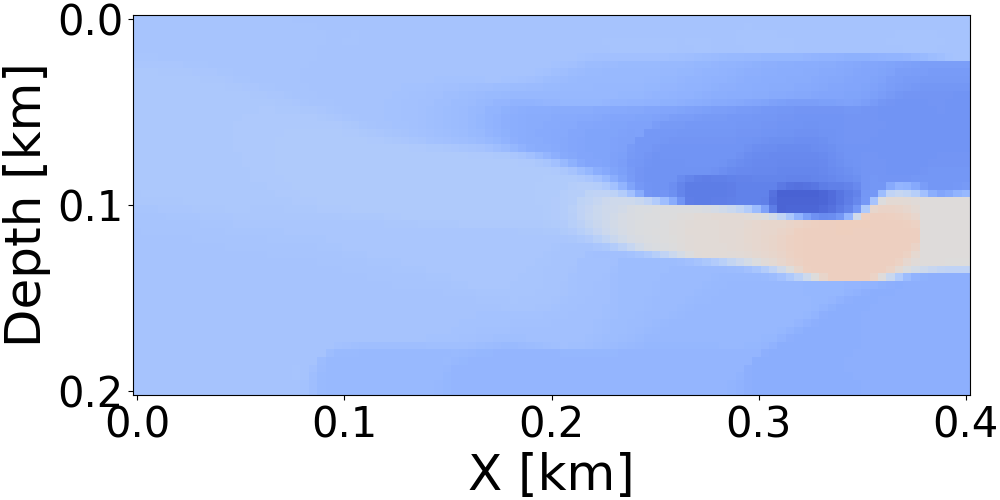
\includegraphics[width=\linewidth]{public/alpha_150}
%            \vspace{-6mm}
            \caption*{(b) Proposed, $\alpha$ = 150}
%            \vspace{1mm}
        \end{minipage} &
        \hspace{-13mm}
        \begin{minipage}[b]{\linewidth}
            \centering
            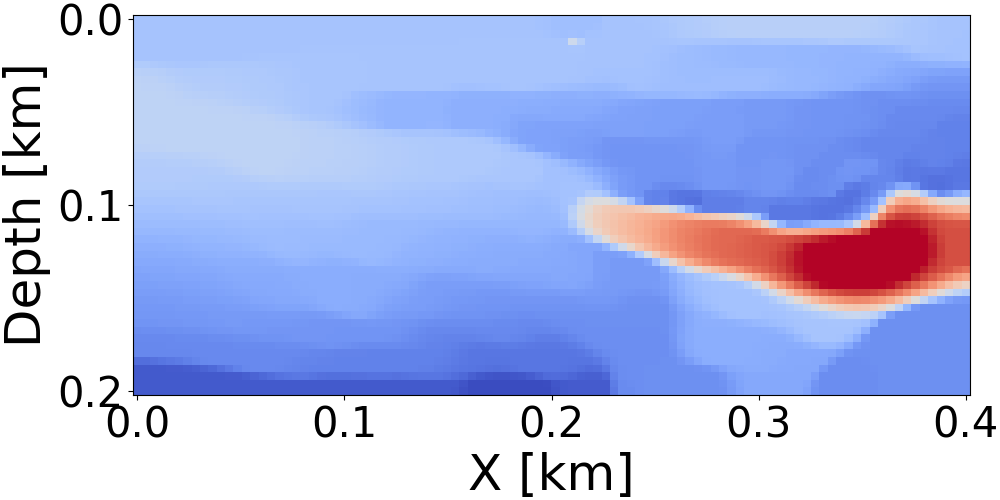
\includegraphics[width=\linewidth]{public/alpha_350}
%            \vspace{-6mm}
            \caption*{(c) Proposed, $\alpha$ = 350}
%            \vspace{1mm}
        \end{minipage} &
        \hspace{-18mm}
        \begin{minipage}[b]{\linewidth}
            \centering
            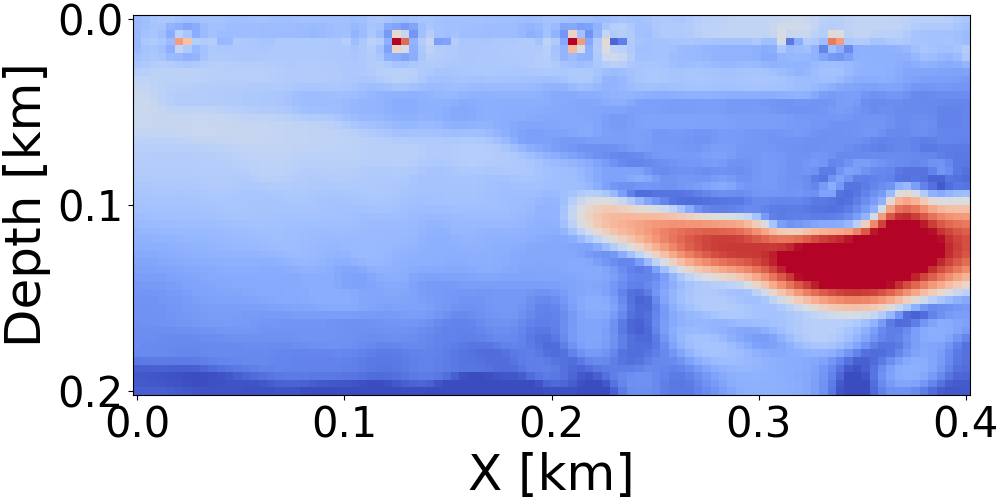
\includegraphics[width=\linewidth]{public/alpha_550}
%            \vspace{-6mm}
            \caption*{(d) Proposed, $\alpha$ = 550}
%            \vspace{1mm}
        \end{minipage} &
%        \hspace{-18mm}
%        \multirow[t]{3}{*}{\raisebox{-5mm}{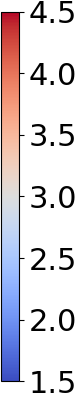
\includegraphics[height=20mm]{public/color-bar}}} \\
    \end{tabular}
%    \vspace{-3mm}
    \captionsetup{margin=1cm}
    \caption{
        Velocity models [km/s] and their corresponding reconstructions. (c) is the best reconstruction result. \\
        (b) is over-smoothed with a stronger TV constraint, and (d) similar results to (a) with a weaker one.
    }
%    \vspace{-4mm}
    \vspace{1mm}
    \label{fig:velocity-models-pure}
\end{figure*}

\begin{figure*}[htbp]
    \centering
    \begin{tabular}{m{43mm} m{43mm} m{43mm} m{43mm} m{10mm}}
        \hspace{-3mm}
        \begin{minipage}[b]{\linewidth}
            \centering
            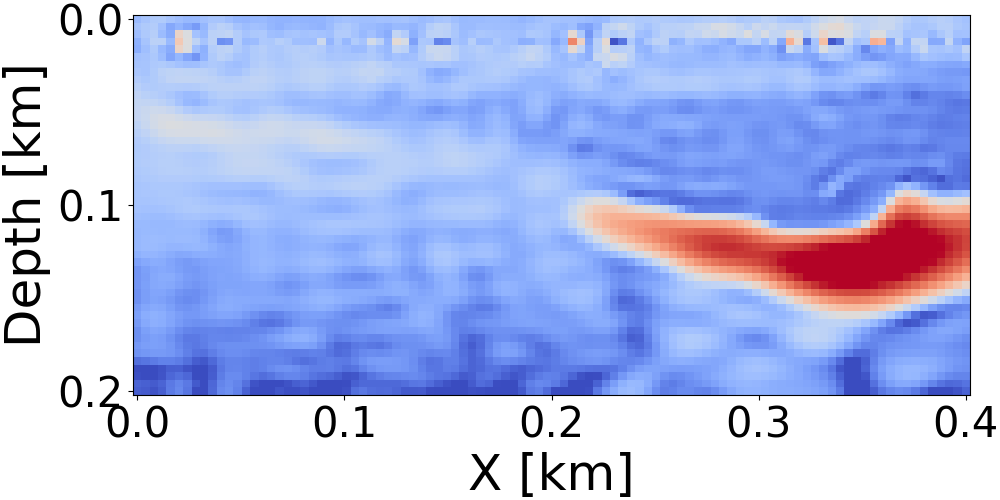
\includegraphics[width=\linewidth]{public/gradient_noisy}
%            \vspace{-6mm}
            \caption*{(e) Standard FWI}
%            \vspace{1mm}
        \end{minipage} &
        \hspace{-8mm}
        \begin{minipage}[b]{\linewidth}
            \centering
            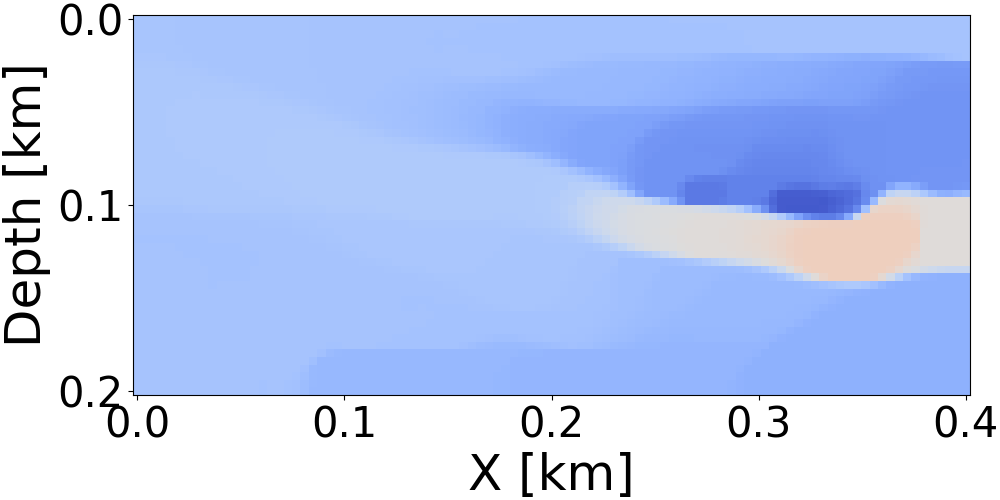
\includegraphics[width=\linewidth]{public/alpha_150_noisy}
%            \vspace{-6mm}
            \caption*{(f) Proposed, $\alpha$ = 150}
%            \vspace{1mm}
        \end{minipage} &
        \hspace{-13mm}
        \begin{minipage}[b]{\linewidth}
            \centering
            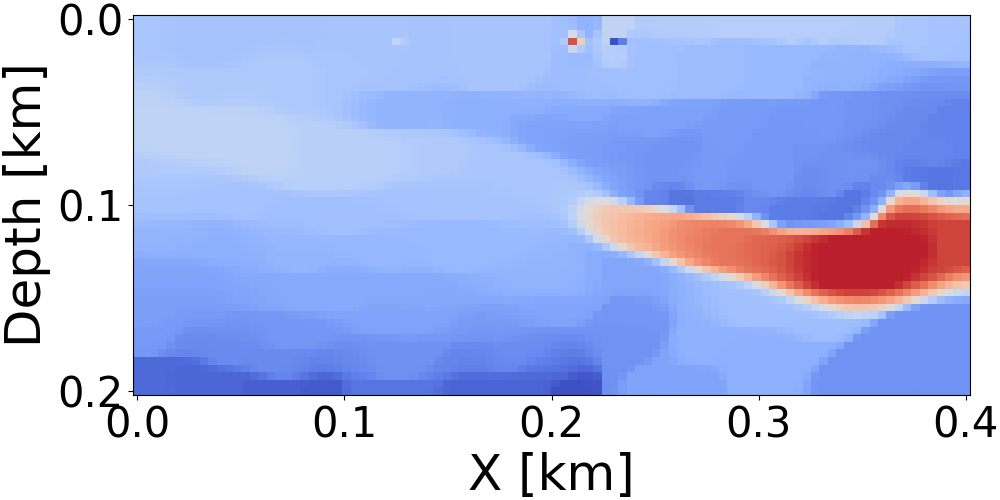
\includegraphics[width=\linewidth]{public/alpha_350_noisy}
%            \vspace{-6mm}
            \caption*{(g) Proposed, $\alpha$ = 350}
%            \vspace{1mm}
        \end{minipage} &
        \hspace{-18mm}
        \begin{minipage}[b]{\linewidth}
            \centering
            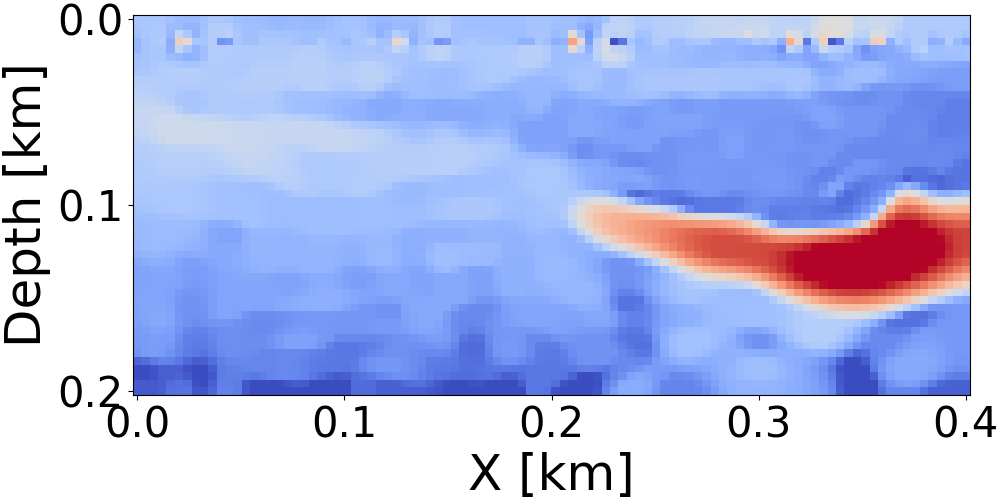
\includegraphics[width=\linewidth]{public/alpha_550_noisy}
%            \vspace{-6mm}
            \caption*{(h) Proposed, $\alpha$ = 550}
%            \vspace{1mm}
        \end{minipage} &
        \hspace{-21.5mm}
        \multirow[t]{3}{*}{\raisebox{-2.3mm}{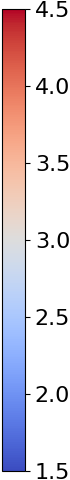
\includegraphics[height=40mm]{public/color-bar-min}}} \\
    \end{tabular}
%    \vspace{-3mm}
    \captionsetup{margin=1cm}
    \caption{
        Velocity models [km/s] and their corresponding reconstructions (with the noisy data). Similar to Fig.~\ref{fig:velocity-models-pure}, (g) is the best result, and (f)/(h) are the results with stronger/weaker TV constraint.
    }
    \vspace{3mm}
    \label{fig:velocity-models-noisy}
\end{figure*}

\begin{figure*}[htbp]
    \centering
    \hspace{-3mm}
%    \begin{minipage}{58mm}
%        \centering
%        \includegraphics[width=\linewidth]{public/iters-ssim}
%%        \vspace{-6mm}
%        \caption{SSIM against iters.}
%        \label{fig:iters-ssim}
%        \vspace{-2mm}
%    \end{minipage}
%    \hspace{-1mm}
    \begin{minipage}{58mm}
        \centering
        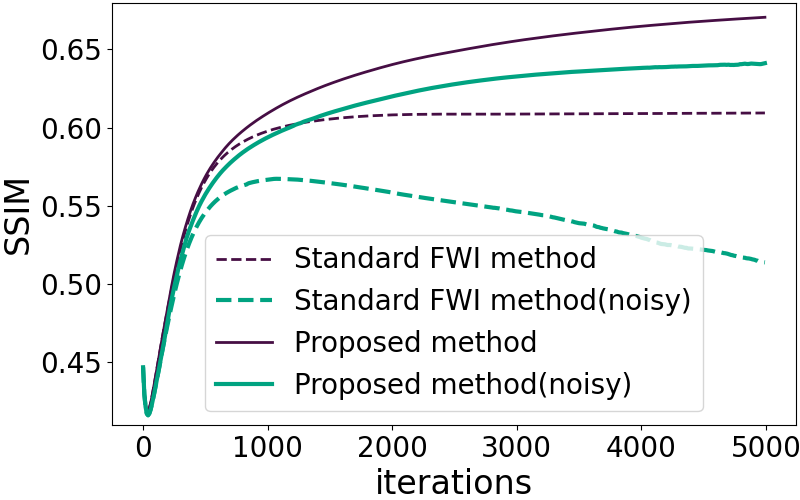
\includegraphics[width=\linewidth]{public/iters-ssim-all-colored}
%        \vspace{-6mm}
        \caption{SSIM against iters ($\alpha$ = 350).}
        \label{fig:iters-ssim-noisy}
%        \vspace{-5mm}
        \vspace{3mm}
    \end{minipage}
    \hspace{-1mm}
    \begin{minipage}{58mm}
        \centering
        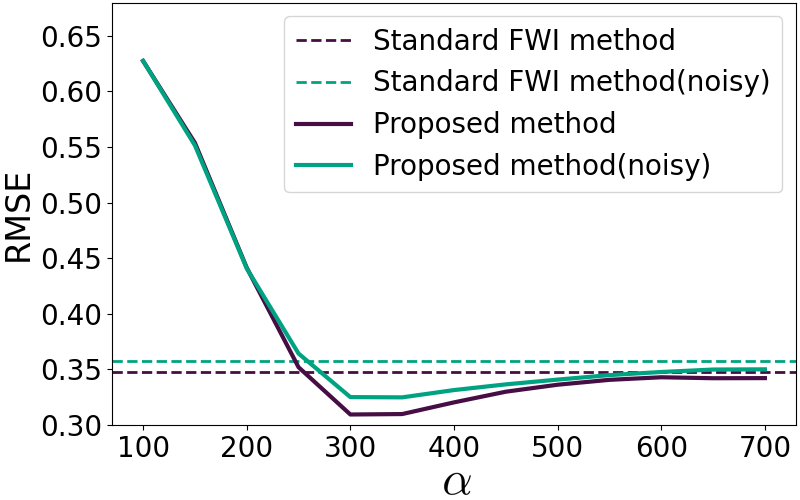
\includegraphics[width=\linewidth]{public/alpha-rmse-colored}
%        \vspace{-6mm}
        \caption{RMSE against $\alpha$.}
        \label{fig:alpha-rmse}
%        \vspace{-5mm}
        \vspace{3mm}
    \end{minipage}
    \hspace{-2mm}
    \begin{minipage}{58mm}
        \centering
        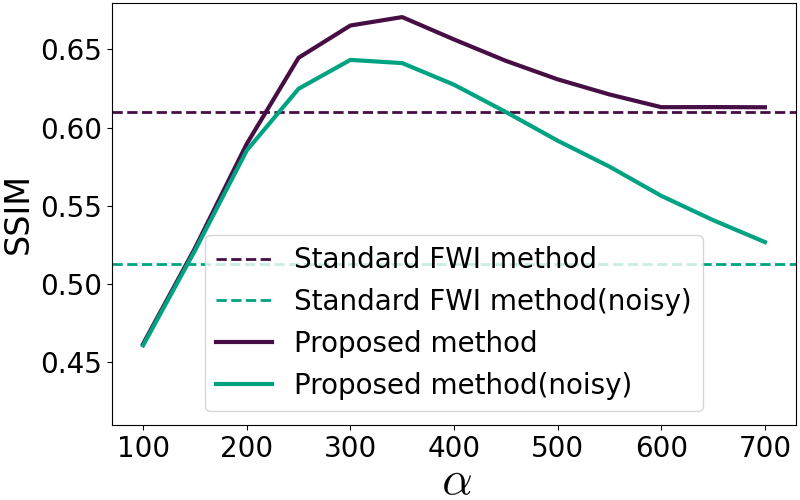
\includegraphics[width=\linewidth]{public/alpha-ssim-colored}
%        \vspace{-6mm}
        \caption{SSIM against $\alpha$.}
        \label{fig:alpha-ssim}
%        \vspace{-3mm}
        \vspace{3mm}
    \end{minipage}
\end{figure*}





\subsection{Results and Discussion} \label{subsec:results-and-discussion}
First, we present the experimental results without noise in the observed seismic data.
Fig.~\ref{fig:velocity-models-pure} shows the reconstructed velocity models using the standard FWI method and the proposed methods with $\alpha$ = 150, 350, and 550.
The best parameter is $\alpha$ = 350, where $\alpha$ = 150 represents a stronger TV constraint and $\alpha$ = 550 represents a weaker one.
The standard FWI method generates wave-like artifacts throughout.
In contrast, our proposed method with the best parameter, which is $\alpha$ = 350, achieves the accurate velocity model reconstruction without these artifacts.
As shown in Fig.~\ref{fig:alpha-rmse} and Fig.~\ref{fig:alpha-ssim}, the proposed method archive accurate reconstruction performance, as evidenced by quantitative evaluations using the Root Mean Squared Error (RMSE) and the Structural Similarity Index Measure (SSIM).
The case of $\alpha$ = 150, 550 will be discussed later.

%For quantitative evaluation, Fig.~\ref{fig:iters-ssim} shows the Structural Similarity Index Measure (SSIM) against the number of iterations for our proposed method and the standard FWI method.
%The proposed method consistently achieves higher SSIM values than the standard FWI method at every iteration, indicating enhanced reconstruction accuracy.

Second, we present the experimental results with the noisy observed seismic data.
Fig.~\ref{fig:velocity-models-noisy} shows the reconstructed velocity models using the standard FWI method and the proposed methods with $\alpha$ = 150, 350 and 550.
In the FWI problem with the noisy observed seismic data, the standard FWI method generates stronger wave-like artifacts throughout.
In contrast, our proposed method with $\alpha$ = 350 as the appropriate parameter still achieves accurate velocity model reconstruction without these artifacts and achieves almost the same level of performance as in the noiseless case.
This demonstrates the robustness of the reconstruction accuracy to noise in the observed seismic data.

Fig.~\ref{fig:iters-ssim-noisy} shows the SSIM against the number of iterations for our proposed method and the standard FWI method.
The standard FWI method with the noisy observed seismic data degrades the SSIM after a certain number of iterations.
On the other hand, the proposed method maintains a consistently high value without degrading the SSIM even after a large number of iterations.
This shows that the proposed method effectively reduces the risk of overfitting to noisy data, providing stable and accurate performance even as the number of iterations increases.

For a more detailed analysis of the TV constraint parameter $\alpha$, we plot the RMSE and SSIM of our proposed method against the parameter $\alpha$ and the standard FWI method in Fig.~\ref{fig:alpha-rmse} and Fig.~\ref{fig:alpha-ssim}.
When around $\alpha$ = 350, the proposed method achieves the best RMSE and SSIM.
When $\alpha$ is smaller, the TV constraint becomes stronger, the RMSE and SSIM worsens, and over-smoothing occurs, as in Fig.~\ref{fig:velocity-models-pure} and Fig.~\ref{fig:velocity-models-noisy} for $\alpha$ = 150.
On the other hand, when $\alpha$ is larger, the TV constraint becomes weaker and the result is similar to the standard FWI method, as in Fig.~\ref{fig:velocity-models-pure} and Fig.~\ref{fig:velocity-models-noisy} for $\alpha$ = 550.
However, thanks to the box constraint, the proposed method still outperforms the standard FWI method.
This demonstrates that the parameter $\alpha$ has a clear and predictable effect on the reconstructed velocity model, which can be easily adjusted to achieve accurate results.



    \section{Conclusion}        \label{sec:Conclusion}      In this paper, we developed an efficient algorithm to solve the TV and box constrained FWI problem based on PDS.
Our algorithm does not require approximations when incorporating the constraints, leading to more accurate reconstructions.
Furthermore, the algorithm significantly enhances computational efficiency without inner loops.
Experimental results demonstrate that our method successfully eliminates wave-like artifacts and noise present in the standard FWI method, resulting in a more accurate velocity model and a superior RMSE and SSIM value regardless of the presence of noise in the observed seismic data.


    \ifCLASSOPTIONcaptionsoff
      \newpage
    \fi

    \newpage

    \begin{spacing}{1}
        \small
        \bibliographystyle{IEEEtranN}
        \bibliography{references}
    \end{spacing}
\end{document}